\chapter{play us a tune pal}
\label{sec:listing}
\lstset{style=68KStyle}

Music in \textit{Tempest 2000} comes in the form of \icode{mod} files. The mechanics of
processing these files are hidden from us in a blob of bytes provide by Imagitec Ltd
and included in the game binary. This blob of bytes is a sound synthesiser that transforms
the contents of a \icode{mod} file into a tune that you can hear with your ears. What we can
do instead is dig into the contents and structure of a mod file to understand how it stores
a tune. The obvious candidate for this research is the music played over the title screen.

I'm not sure if this music ever had a proper title, however the source code knows it fondly
as \icode{tune13.mod}. This file, along with all the other tunes included in the game, are
stored in a reference table called \icode{modbase}. This allows us to pick a tune for playing
by referencing it using an index into the table. 

\begin{lstlisting}
modbase      EQU $8d6800
modtable:
.dc.l modbase + $100   ; tune13.mod
.dc.l modbase + $18d2c ; tune7.mod
.dc.l modbase + $37a04 ; tune1.mod
.dc.l modbase + $5bd7c ; tune3.mod
.dc.l modbase + $80b22 ; rave4.mod
.dc.l modbase + $99d72 ; tune5.mod
.dc.l modbase + $b0a50 ; tune12.mod
.dc.l 0
\end{lstlisting}

In the little routine that plays a selected tune we can see this happening in practice. The
index value for the selected tune is passed in the \icode{d0} register and used as an index
into \icode{modbase} to retrieve the address in memory of the tune we've picked to play.
\clearpage
\begin{lstlisting}
playtune:
        jsr STOP_MOD               ; Stop any current tune.
        lsl #2,d0                  ; Multiply index (d0) by 4
        lea modbase,a0             ; Point a0 at modbase.
        move.l 0(a0,d0.w),a0       ; Get tune base using index.
        jsr PT_MOD_INIT            ; Point the MOD player at a0.
        move.b vols,d0             ; Store the volume in d0.
        and.l #$ff,d0              ; Keep it between 0 and 255
        clr d1                     ; Clear d1
        jsr SET_VOLUME             ; Actually set the volume.
        move.l d0,vset             ; Store the selected volume.
        jsr NOFADE                 ; Turn off 'fading'.
        jmp START_MOD              ; Start playing the tune.
\end{lstlisting}

So to play the title screen tune, which is the first entry in \icode{modtable}, we point
the sound synthesiser at the region in memory containing \icode{tune13.mod} by calling
its black-box routine \icode{PT\_MOD\_INIT} and then once we've set the volume, instruct
it to start playing the darn thing (\icode{jmp START\_MOD}).

To understand the contents of \icode{tune13.mod} and how it gives us a tune, it is best to
start with the most basic building blocks it contains. These are 11 raw sound samples of
Pulse Code Modulation (PCM) data like the ones we discussed in 
\hyperref[sec:sexy_yes]{\textcolor{blue}{'sexy yes'}}.
They are stored at the very end of the file, one after another from
byte 9276 to byte 101416. This means they constitute the bulk of the \icode{tune13.mod} tune file - which
is not surprising since they are the part of the file that carries all the sounds. If you want to hear
what each sample sounds like, your reader might support clicking on each sample to play it.

\begin{figure}[H]
{
    \begin{subfigure}{0.23\textwidth}
      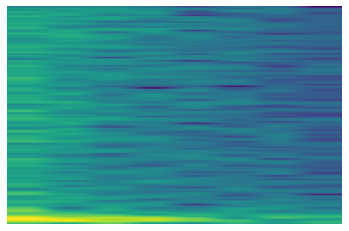
\includegraphics[width=3cm]{titletune/buttons/samples/tune13.mod-1.wav-spec.png}%
      \makebox[0pt][r]{%
        \raisebox{.3cm}{%
          \textattachfile{src/titletune/samples/tune13.mod-1.wav}{
\includegraphics[width=1.5cm]{sounds/play.png}}%
        }\hspace*{0.75cm}%
      }%
      \caption*{Sample 1}
    \end{subfigure}
    \begin{subfigure}{0.23\textwidth}
      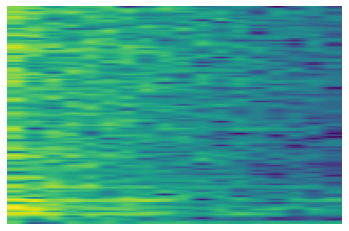
\includegraphics[width=3cm]{titletune/buttons/samples/tune13.mod-2.wav-spec.png}%
      \makebox[0pt][r]{%
        \raisebox{.3cm}{%
          \textattachfile{src/titletune/samples/tune13.mod-2.wav}{
\includegraphics[width=1.5cm]{sounds/play.png}}%
        }\hspace*{0.75cm}%
      }%
      \caption*{Sample 2}
    \end{subfigure}
    \begin{subfigure}{0.23\textwidth}
      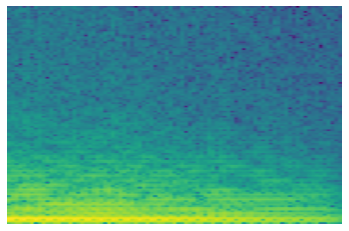
\includegraphics[width=3cm]{titletune/buttons/samples/tune13.mod-4.wav-spec.png}%
      \makebox[0pt][r]{%
        \raisebox{.3cm}{%
          \textattachfile{src/titletune/samples/tune13.mod-4.wav}{
\includegraphics[width=1.5cm]{sounds/play.png}}%
        }\hspace*{0.75cm}%
      }%
      \caption*{Sample 4}
    \end{subfigure}
    \begin{subfigure}{0.23\textwidth}
      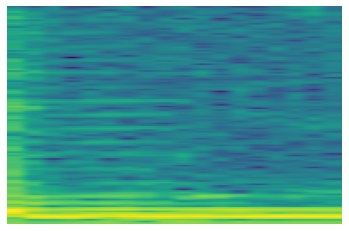
\includegraphics[width=3cm]{titletune/buttons/samples/tune13.mod-5.wav-spec.png}%
      \makebox[0pt][r]{%
        \raisebox{.3cm}{%
          \textattachfile{src/titletune/samples/tune13.mod-5.wav}{
\includegraphics[width=1.5cm]{sounds/play.png}}%
        }\hspace*{0.75cm}%
      }%
      \caption*{Sample 5}
    \end{subfigure}
    \begin{subfigure}{0.24\textwidth}
      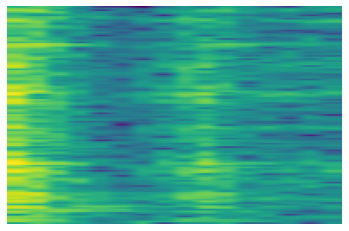
\includegraphics[width=3cm]{titletune/buttons/samples/tune13.mod-6.wav-spec.png}%
      \makebox[0pt][r]{%
        \raisebox{.3cm}{%
          \textattachfile{src/titletune/samples/tune13.mod-6.wav}{
\includegraphics[width=1.5cm]{sounds/play.png}}%
        }\hspace*{0.75cm}%
      }%
      \caption*{Sample 6}
    \end{subfigure}
    \begin{subfigure}{0.24\textwidth}
      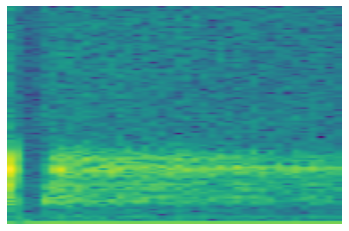
\includegraphics[width=3cm]{titletune/buttons/samples/tune13.mod-7.wav-spec.png}%
      \makebox[0pt][r]{%
        \raisebox{.3cm}{%
          \textattachfile{src/titletune/samples/tune13.mod-7.wav}{
\includegraphics[width=1.5cm]{sounds/play.png}}%
        }\hspace*{0.75cm}%
      }%
      \caption*{Sample 7}
    \end{subfigure}
    \begin{subfigure}{0.24\textwidth}
      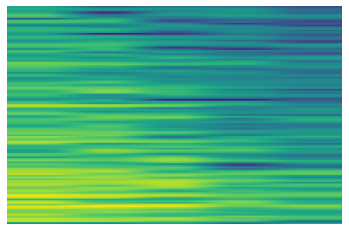
\includegraphics[width=3cm]{titletune/buttons/samples/tune13.mod-8.wav-spec.png}%
      \makebox[0pt][r]{%
        \raisebox{.3cm}{%
          \textattachfile{src/titletune/samples/tune13.mod-8.wav}{
\includegraphics[width=1.5cm]{sounds/play.png}}%
        }\hspace*{0.75cm}%
      }%
      \caption*{Sample 8}
    \end{subfigure}
    \begin{subfigure}{0.24\textwidth}
      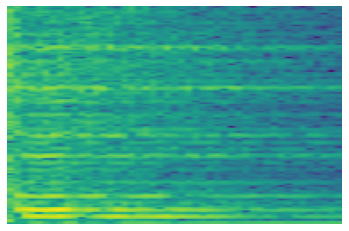
\includegraphics[width=3cm]{titletune/buttons/samples/tune13.mod-10.wav-spec.png}%
      \makebox[0pt][r]{%
        \raisebox{.3cm}{%
          \textattachfile{src/titletune/samples/tune13.mod-10.wav}{
\includegraphics[width=1.5cm]{sounds/play.png}}%
        }\hspace*{0.75cm}%
      }%
      \caption*{Sample 10}
    \end{subfigure}
}
\end{figure}
\clearpage

\begin{figure}[H]
{
    \begin{subfigure}{0.25\textwidth}
      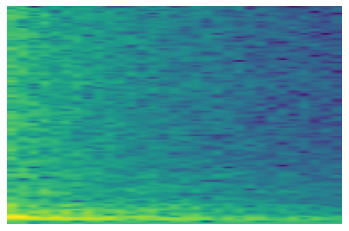
\includegraphics[width=3cm]{titletune/buttons/samples/tune13.mod-11.wav-spec.png}%
      \makebox[0pt][r]{%
        \raisebox{.3cm}{%
          \textattachfile{src/titletune/samples/tune13.mod-11.wav}{
\includegraphics[width=1.5cm]{sounds/play.png}}%
        }\hspace*{0.75cm}%
      }%
      \caption*{Sample 11}
    \end{subfigure}
    \begin{subfigure}{0.25\textwidth}
      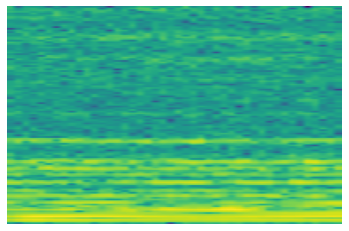
\includegraphics[width=3cm]{titletune/buttons/samples/tune13.mod-12.wav-spec.png}%
      \makebox[0pt][r]{%
        \raisebox{.3cm}{%
          \textattachfile{src/titletune/samples/tune13.mod-12.wav}{
\includegraphics[width=1.5cm]{sounds/play.png}}%
        }\hspace*{0.75cm}%
      }%
      \caption*{Sample 12}
    \end{subfigure}
    \begin{subfigure}{0.25\textwidth}
      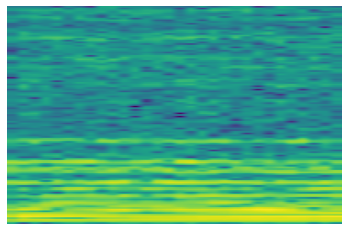
\includegraphics[width=3cm]{titletune/buttons/samples/tune13.mod-13.wav-spec.png}%
      \makebox[0pt][r]{%
        \raisebox{.3cm}{%
          \textattachfile{src/titletune/samples/tune13.mod-13.wav}{
\includegraphics[width=1.5cm]{sounds/play.png}}%
        }\hspace*{0.75cm}%
      }%
      \caption*{Sample 13}
    \end{subfigure}
}\caption*{All 11 sound samples and their spectrograms. If your reader supports it you can play the samples.}
\end{figure}

If you try playing the files you'll notice that the majority of them are single notes on an instrument. This
gives us a clue as to what the rest of the \icode{tune13.mod} file might contain: instructions on how to play
these notes in the correct order. More than this, the instructions might even tell us what pitch to play each
note at, for example, whether a C sharp or a B flat.

We find these instructions at byte 1084 in the file and they occupy all the space in the file up to the beginning
of the samples at byte 9276. The instructions are broken up into chunks called 'Patterns'. Each 'Pattern' describes
a passage of music, using the samples to play notes across four separate audio channels at once. Another way of thinking
of a 'Pattern' is like a piece of sheet music that describes the notes to play and the instrument to play them for four
different players. In this case our instruments are the 'samples'. To give you an idea of what I mean here is the
first note for all four players (which we call channels) given in the first 16 bytes of the data for the first of
the seven patterns in \icode{tune13.mod}.

\begin{figure}[H]
  {
    \setlength{\tabcolsep}{3.0pt}
    \setlength\cmidrulewidth{\heavyrulewidth} % Make cmidrule = 
    \begin{adjustbox}{width=7cm,center}

      \begin{tabular}{lllll}
        \toprule
	 & Bytes & Sample & Note & Effect \\
        \midrule
	Channel 1 & \icode{007f1000} & 1 & A3 &  \\
	Channel 2 & \icode{01944f09} & 4 & C\#2 & Set Speed 09\\
	Channel 3 & \icode{011d5000} & 5 & G2 &  \\
	Channel 4 & \icode{00000000} & &   &   \\
      \end{tabular}
    \end{adjustbox}
  }\caption*{Decoding the first 16 bytes (4 per channel) in Pattern 000.}
\end{figure}

One the following page we see the complete decoded set of instructions contained in Pattern 000. As you look through it you can get
a sense of the note being played on each channel and the instrument used, along with any special instruction (effect)
specified. 

\begin{figure}[H]
  {
    \setlength{\tabcolsep}{3.0pt}
    \setlength\cmidrulewidth{\heavyrulewidth} % Make cmidrule = 
    \begin{adjustbox}{width=11cm,center}
      \begin{tabular}{llllllllllll}
        \toprule
Channel 1 &  &  & Channel 2 &  &  & Channel 3 &  &  & Channel 4 &  &  \\
Sample & Note & Effect & Sample & Note & Effect & Sample & Note & Effect & Sample & Note & Effect \\
        \midrule
1 & A3 &   & 4 & C\#2 & Set Speed 09 & 5 & G2 &   &   &   &   \\
8 & A\#3 &   &   &   &   & 5 & G2 & Set Volume 15 &   &   &   \\
6 & A3 &   &   &   &   & 5 & G2 &   &   &   &   \\
6 & A3 &   &   &   &   & 5 & G2 & Set Volume 25 &   &   &   \\
8 & A\#3 &   &   &   &   &   &   &   &   &   &   \\
8 & A\#3 &   &   &   &   & 5 & G2 & Set Volume 15 &   &   &   \\
6 & A3 &   &   &   &   & 5 & G2 &   &   &   &   \\
1 & A3 &   &   &   &   & 5 & G2 & Set Volume 25 &   &   &   \\
2 & D3 &   &   &   &   &   &   &   &   &   &   \\
8 & B3 &   &   &   &   & 5 & G2 & Set Volume 15 &   & G2 &   \\
8 & B3 &   &   &   &   & 5 & G2 &   & 10 & D3 &   \\
6 & A3 &   &   &   &   & 5 & G2 & Set Volume 25 & 10 & G2 &   \\
0 &   &   &   &   &   &   &   &   & 10 & D3 &   \\
8 & B3 &   &   &   &   & 5 & G2 & Set Volume 15 & 10 & G2 &   \\
6 & A3 &   &   &   &   & 5 & G2 &   & 10 & D\#3 &   \\
1 & A3 &   &   &   &   & 5 & G2 & Set Volume 25 & 10 & D3 &   \\
1 & A3 &   &   &   &   &   &   &   &   &   &   \\
8 & B3 &   &   &   &   & 5 & G2 & Set Volume 15 &   &   &   \\
6 & A3 &   &   &   &   & 5 & G2 &   &   &   &   \\
6 & A3 &   &   &   &   & 5 & G2 & Set Volume 25 &   &   &   \\
8 & A\#3 &   &   &   &   &   &   &   &   &   &   \\
8 & A\#3 &   &   &   &   & 5 & G2 & Set Volume 15 &   &   &   \\
6 & A3 &   &   &   &   & 5 & G2 &   &   &   &   \\
1 & A3 &   &   &   &   & 5 & G2 & Set Volume 25 &   &   &   \\
2 & D3 &   &   &   &   &   &   &   &   &   &   \\
0 &   &   &   &   &   & 5 & G2 & Set Volume 15 &   &   &   \\
6 & A3 &   &   &   &   & 5 & G2 &   &   & F2 &   \\
6 & A3 &   &   &   &   & 5 & G2 & Set Volume 25 &   &   &   \\
8 & A\#3 &   &   &   &   &   &   &   &   &   &   \\
8 & A\#3 &   & 4 & D2 &   & 5 & F2 & Set Volume 15 &   & F2 &   \\
6 & A3 &   &   &   &   & 5 & F2 &   &   &   &   \\
1 & A3 &   &   &   &   & 5 & F2 & Set Volume 25 &   &   &   \\
1 & A3 &   & 4 & C\#2 &   &   &   &   &   & F2 &   \\
8 & A\#3 &   &   &   &   & 5 & G2 & Set Volume 15 &   & G2 &   \\
6 & A3 &   &   &   &   & 5 & G2 &   &   &   &   \\
6 & A3 &   &   &   &   & 5 & G2 & Set Volume 25 &   &   &   \\
8 & A\#3 &   &   &   &   &   &   &   &   &   &   \\
8 & A\#3 &   &   &   &   & 5 & G2 & Set Volume 15 &   &   &   \\
6 & A3 &   &   &   &   & 5 & G2 &   &   &   &   \\
1 & A3 &   &   &   &   & 5 & G2 & Set Volume 25 &   &   &   \\
2 & D3 &   &   &   &   &   &   &   &   &   &   \\
0 &   &   &   &   &   & 5 & G2 & Set Volume 15 &   &   &   \\
6 & A3 &   &   &   &   & 5 & G2 &   &   & D3 &   \\
6 & A3 &   &   &   &   & 5 & G2 & Set Volume 25 &   & G2 &   \\
8 & A\#3 &   &   &   &   &   &   &   &   & D3 &   \\
8 & A\#3 &   &   &   &   & 5 & G2 & Set Volume 15 &   & G2 &   \\
6 & A3 &   &   &   &   & 5 & G2 &   &   & D\#3 &   \\
1 & A3 &   &   &   &   & 5 & G2 & Set Volume 25 &   & B2 &   \\
1 & A3 &   &   &   &   &   &   &   &   &   &   \\
8 & A\#3 &   &   &   &   & 5 & G2 & Set Volume 15 &   &   &   \\
6 & A3 &   &   &   &   & 5 & G2 &   &   &   &   \\
6 & A3 &   &   &   &   & 5 & G2 & Set Volume 25 &   &   &   \\
8 & A\#3 &   &   &   &   &   &   &   &   &   &   \\
8 & A\#3 &   &   &   &   & 5 & G2 & Set Volume 15 &   &   &   \\
6 & A3 &   &   &   &   & 5 & G2 &   &   &   &   \\
1 & A3 &   &   &   &   & 5 & G2 & Set Volume 25 &   &   &   \\
2 & D3 &   &   &   &   &   &   &   &   &   &   \\
0 &   &   &   &   &   & 5 & G2 & Set Volume 15 &   &   &   \\
6 & A3 &   &   &   &   & 5 & G2 &   &   &   &   \\
6 & A3 &   &   &   &   & 5 & G2 & Set Volume 25 &   &   &   \\
8 & A\#3 &   &   &   &   &   &   &   &   &   &   \\
1 & A3 &   &   &   &   & 5 & G2 & Set Volume 15 &   &   &   \\
6 & A3 &   &   &   &   & 5 & G2 &   &   &   &   \\
1 & A3 &   &   &   &   & 5 & G\#2 & Set Volume 25 &   &   &   \\
        \bottomrule
      \end{tabular}
    \end{adjustbox}
  }\caption*{Decoding the full instructions for Pattern 000.}
\end{figure}
What if we attempted to turn the notes in Pattern 0 into some sheet music? It's just a question
of representing each channel as a stave and transcribing the notes from the pattern. We can't 
display the sample that's being used to play the note, but we do get a sense of the music
that's being played. 

\begin{figure}[H]
  \centering
        
\includegraphics[width=10cm]{src/titletune/sheet_music/title_no_0_page_1001.png}%
  \caption*{Pattern 0 rendered as sheet music.}
\end{figure}


With a single chunk of music like this we now have the makings of a tune, built up from using our samples in a series of 
machine-readable sheet music instructions in a pattern.

 Our next step is to come up with as many of these patterns
as we need to form a complete tune. In theory we could mix and match the patterns in any sequence we like and play
them one after the other to form the finished article. In the 
case of \icode{tune13.mod}, the structure is quite simple. At byte 952 in our \icode{tune13.mod} file we list the
order in which the patterns are to be played. This also lets us know how many patterns in total the file contains.
The full list is: 0, 1, 2, 3, 4, 3, 6, 7, 5. With this information we can illustrate the title tune in its
entirety by piecing together the transcriptions of each of the patterns. 
 
\begin{figure}[H]
{
    \begin{subfigure}{0.43\textwidth}
        
\includegraphics[width=6cm]{src/titletune/sheet_music/title_no_0_page_1001.png}%
      \caption*{Pattern 0}
    \end{subfigure}
    \begin{subfigure}{0.43\textwidth}
        
\includegraphics[width=6cm]{src/titletune/sheet_music/title_no_1_page_1001.png}%
      \caption*{Pattern 1}
    \end{subfigure}
    \begin{subfigure}{0.43\textwidth}
        
\includegraphics[width=6cm]{src/titletune/sheet_music/title_no_2_page_1001.png}%
      \caption*{Pattern 2}
    \end{subfigure}
    \begin{subfigure}{0.43\textwidth}
        
\includegraphics[width=6cm]{src/titletune/sheet_music/title_no_3_page_1001.png}%
      \caption*{Pattern 3}
    \end{subfigure}
    \begin{subfigure}{0.43\textwidth}
        
\includegraphics[width=6cm]{src/titletune/sheet_music/title_no_4_page_1001.png}%
      \caption*{Pattern 4}
    \end{subfigure}
    \hspace{1.5cm}
    \begin{subfigure}{0.43\textwidth}
        
\includegraphics[width=6cm]{src/titletune/sheet_music/title_no_3_page_1001.png}%
      \caption*{Pattern 3}
    \end{subfigure}
}
\end{figure}

\begin{figure}[H]
{
    \begin{subfigure}{0.43\textwidth}
        
\includegraphics[width=6cm]{src/titletune/sheet_music/title_no_6_page_1001.png}%
      \caption*{Pattern 6}
    \end{subfigure}
    \begin{subfigure}{0.43\textwidth}
        
\includegraphics[width=6cm]{src/titletune/sheet_music/title_no_7_page_1001.png}%
      \caption*{Pattern 7}
    \end{subfigure}
    \begin{subfigure}{0.43\textwidth}
        
\includegraphics[width=6cm]{src/titletune/sheet_music/title_no_5_page_1001.png}%
      \caption*{Pattern 5}
    \end{subfigure}
}\caption*{The patterns in the order that they're played, giving the complete tune.}
\end{figure}
